\documentclass[12pt,a4paper]{article}

\usepackage{fontawesome5}
\providecommand{\faPencilAlt}{\faIcon{pencil-alt}}

\usepackage{styles/couleurs}
\usepackage{styles/mise_en_page}
\usepackage{styles/boites}
\usepackage{styles/maths}
\usepackage{styles/figures}

\usepackage{enumitem}
\usepackage{array}
\usepackage{tabularx}
\usepackage{amsmath}
\usepackage{amssymb}
\usepackage{tikz}
\usepackage{xparse}
\usepackage{pdflscape}
\usepackage{colortbl}

\usetikzlibrary{calc,arrows.meta,positioning}

\setlist[itemize]{leftmargin=1.4em,itemsep=0.15em,topsep=0.2em}
\setlist[enumerate]{leftmargin=*,itemsep=0.22em,topsep=0.25em}

\newcommand{\lignepointillee}{\noindent\dotfill\par\vspace{0.45em}}

\newcommand{\lignesreponse}[1]{%
\begin{tcolorbox}[
enhanced,colback=white,colframe=NeutreC!40,boxrule=0.5pt,arc=1.5mm,
left=3mm,right=3mm,top=2mm,bottom=1mm,before skip=2pt,after skip=2pt]
\foreach \i in {1,...,#1}{\lignepointillee}
\end{tcolorbox}}

\newcommand{\titreseq}[1]{%
\begin{center}
{\sffamily\large\bfseries\color{SavoirC}#1}
\end{center}}

\newcommand{\grillecent}{%
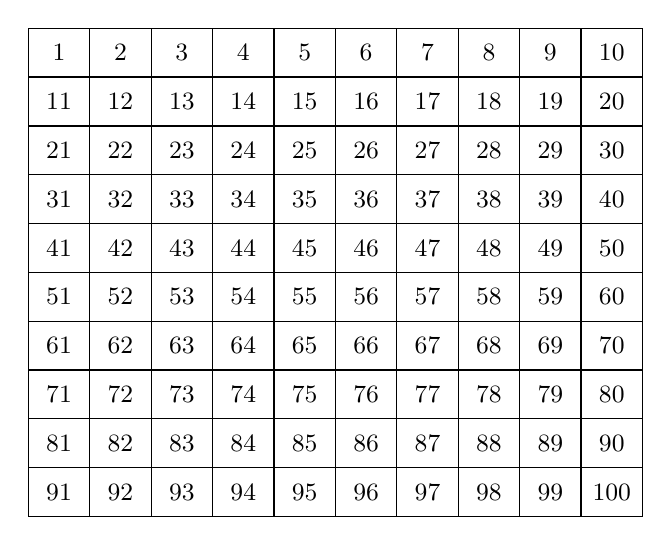
\begin{tikzpicture}[x=0.78cm,y=0.62cm]
  \foreach \n in {1,...,100}{
    \pgfmathtruncatemacro{\col}{mod(\n-1,10)}
    \pgfmathtruncatemacro{\lig}{9-floor((\n-1)/10)}
    \draw[line width=0.45pt] (\col,\lig) rectangle ++(1,1);
    \node[font=\small] at (\col+0.5,\lig+0.5) {\n};
  }
\end{tikzpicture}}

\begin{document}

\titreseq{Activité 4 -- Décomposer un nombre en facteurs premiers}

\remarque{Décomposer un nombre, c'est le remplacer par une expression numérique qui lui est égal. Ici, on s'intéresse aux formes multiplicatives.}

\section*{Partie A -- Deux chemins pour le nombre \(84\)}

Complète les deux arbres.

\begin{center}
\begin{minipage}[t]{0.45\textwidth}
\centering
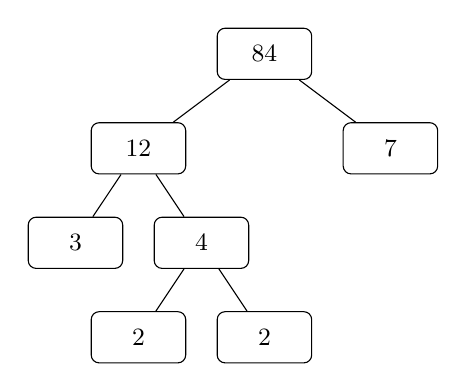
\begin{tikzpicture}[
  level distance=1.2cm,
  level 1/.style={sibling distance=3.2cm},
  level 2/.style={sibling distance=1.6cm},
  every node/.style={draw,rounded corners=1mm,minimum width=1.2cm,
                     minimum height=0.65cm,font=\small}
]
\node {84}
  child {node {12}
    child {node {3}}
    child {node {4}
      child {node {2}}
      child {node {2}}
    }
  }
  child {node {7}};
\end{tikzpicture}

\[
84=\dotfill
\]
\end{minipage}
\hfill
\begin{minipage}[t]{0.45\textwidth}
\centering
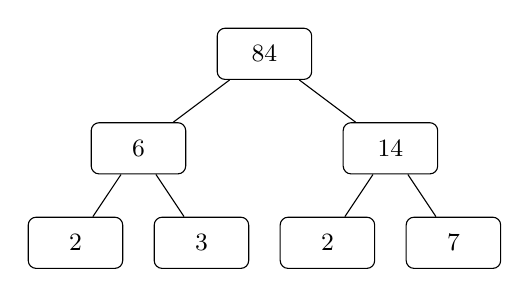
\begin{tikzpicture}[
  level distance=1.2cm,
  level 1/.style={sibling distance=3.2cm},
  level 2/.style={sibling distance=1.6cm},
  every node/.style={draw,rounded corners=1mm,minimum width=1.2cm,
                     minimum height=0.65cm,font=\small}
]
\node {84}
  child {node {6}
    child {node {2}}
    child {node {3}}
  }
  child {node {14}
    child {node {2}}
    child {node {7}}
  };
\end{tikzpicture}

\[
84=\dotfill
\]
\end{minipage}
\end{center}

\begin{enumerate}
  \item Les arbres sont-ils identiques ?
  \item Les facteurs premiers obtenus sont-ils les mêmes ?
  \item Dans quel ordre écrit-on habituellement les facteurs premiers ?
\end{enumerate}

\lignesreponse{4}

\section*{Partie B -- Construire une méthode}

Remets les étapes dans l'ordre.

\begin{itemize}
  \item[\(\square\)] Vérifier le produit obtenu.
  \item[\(\square\)] Choisir un diviseur premier du nombre.
  \item[\(\square\)] Continuer sur le quotient tant qu'il n'est pas premier.
  \item[\(\square\)] Écrire le nombre comme produit de facteurs premiers.
\end{itemize}

\section*{Partie C -- Décomposer}

Décompose chaque nombre en produit de facteurs premiers.
Tu peux utiliser un arbre ou des divisions successives.

\[
60\qquad 90\qquad 126\qquad 150\qquad 196
\]

\lignesreponse{10}

\section*{Partie D -- Vérifier et comparer}

\begin{enumerate}
  \item Vérifie une décomposition en effectuant le produit.
  \item Quels facteurs premiers \(60\) et \(90\) ont-ils en commun ?
  \item Quels facteurs premiers \(126\) et \(196\) ont-ils en commun ?
  \item Une décomposition peut-elle contenir le nombre \(1\) ?
        Justifie.
\end{enumerate}

\lignesreponse{6}

\begin{tcolorbox}[
  enhanced,
  colback=SavoirBg,
  colframe=SavoirC!60,
  boxrule=0.7pt,
  arc=2mm
]
Décomposer un entier en produit de facteurs premiers consiste
à l'écrire comme un produit ne contenant que des nombres premiers.

\[
84=2\times2\times3\times7.
\]
\end{tcolorbox}

\end{document}
